\documentclass[11pt,]{article}
\usepackage{lmodern}
\usepackage{amssymb,amsmath}
\usepackage{ifxetex,ifluatex}
\usepackage{fixltx2e} % provides \textsubscript
\ifnum 0\ifxetex 1\fi\ifluatex 1\fi=0 % if pdftex
  \usepackage[T1]{fontenc}
  \usepackage[utf8]{inputenc}
\else % if luatex or xelatex
  \ifxetex
    \usepackage{mathspec}
  \else
    \usepackage{fontspec}
  \fi
  \defaultfontfeatures{Ligatures=TeX,Scale=MatchLowercase}
\fi
% use upquote if available, for straight quotes in verbatim environments
\IfFileExists{upquote.sty}{\usepackage{upquote}}{}
% use microtype if available
\IfFileExists{microtype.sty}{%
\usepackage{microtype}
\UseMicrotypeSet[protrusion]{basicmath} % disable protrusion for tt fonts
}{}
\usepackage[margin=1in]{geometry}
\usepackage{hyperref}
\hypersetup{unicode=true,
            pdftitle={Quantifying the Trendiness of Trends},
            pdfborder={0 0 0},
            breaklinks=true}
\urlstyle{same}  % don't use monospace font for urls
\usepackage{graphicx,grffile}
\makeatletter
\def\maxwidth{\ifdim\Gin@nat@width>\linewidth\linewidth\else\Gin@nat@width\fi}
\def\maxheight{\ifdim\Gin@nat@height>\textheight\textheight\else\Gin@nat@height\fi}
\makeatother
% Scale images if necessary, so that they will not overflow the page
% margins by default, and it is still possible to overwrite the defaults
% using explicit options in \includegraphics[width, height, ...]{}
\setkeys{Gin}{width=\maxwidth,height=\maxheight,keepaspectratio}
\IfFileExists{parskip.sty}{%
\usepackage{parskip}
}{% else
\setlength{\parindent}{0pt}
\setlength{\parskip}{6pt plus 2pt minus 1pt}
}
\setlength{\emergencystretch}{3em}  % prevent overfull lines
\providecommand{\tightlist}{%
  \setlength{\itemsep}{0pt}\setlength{\parskip}{0pt}}
\setcounter{secnumdepth}{5}
% Redefines (sub)paragraphs to behave more like sections
\ifx\paragraph\undefined\else
\let\oldparagraph\paragraph
\renewcommand{\paragraph}[1]{\oldparagraph{#1}\mbox{}}
\fi
\ifx\subparagraph\undefined\else
\let\oldsubparagraph\subparagraph
\renewcommand{\subparagraph}[1]{\oldsubparagraph{#1}\mbox{}}
\fi

%%% Use protect on footnotes to avoid problems with footnotes in titles
\let\rmarkdownfootnote\footnote%
\def\footnote{\protect\rmarkdownfootnote}

%%% Change title format to be more compact
\usepackage{titling}

% Create subtitle command for use in maketitle
\newcommand{\subtitle}[1]{
  \posttitle{
    \begin{center}\large#1\end{center}
    }
}

\setlength{\droptitle}{-2em}
  \title{Quantifying the Trendiness of Trends}
  \pretitle{\vspace{\droptitle}\centering\huge}
  \posttitle{\par}
  \author{Andreas Kryger Jensen and Claus Thorn Ekstrøm\\
Biostatistics, Institute of Public Health, University of Copenhagen\\
\href{mailto:aeje@sund.ku.dk}{\nolinkurl{aeje@sund.ku.dk}},
\href{mailto:ekstrom@sund.ku.dk}{\nolinkurl{ekstrom@sund.ku.dk}}}
  \preauthor{\centering\large\emph}
  \postauthor{\par}
  \predate{\centering\large\emph}
  \postdate{\par}
  \date{26 December, 2019}

\usepackage{bm}
\usepackage{amssymb}
\usepackage[labelfont=bf]{caption}
\DeclareMathOperator*{\argsup}{arg\,sup}
\DeclareMathOperator*{\argmin}{arg\,min}
\DeclareMathOperator*{\E}{E}
\DeclareMathOperator*{\Cov}{Cov}
\DeclareMathOperator*{\Cor}{Cor}
\DeclareMathOperator*{\Var}{Var}
\DeclareMathOperator*{\Erf}{Erf}
\DeclareMathOperator*{\Erfc}{Erfc}
\usepackage{multirow}
\usepackage[amsthm,thmmarks]{ntheorem}
\newtheorem{definition}{Definition}
\newtheorem{assumption}{Assumption}
\newtheorem{proposition}{Proposition}
\theoremstyle{nonumberplain}
\newtheorem{Proof}{Proof}

\begin{document}
\maketitle

\begin{abstract}
A statement often seen in the news concerning some public health outcome is that some trend has changed or been broken. Such statements are often based on longitudinal data from surveys, and the change in trend is claimed to have occurred at the time of the latest data collection. These types of statistical assessments are very important as they may potentially influence public health decisions on a national level.

We propose two measures for quantifying the trendiness of trends. Under the assumption that reality evolves in continuous time we define what constitutes a trend and a change in a trend, and we introduce a probabilistic Trend Direction Index. This index has the interpretation of the probability that a latent characteristic has changed monotonicity at any given time conditional on observed data. We also define a global index of Expected Trend Instability quantifying the expected number of times that a trend has changed on an interval.

Using a latent Gaussian process model we show how the Trend Direction Index and the Expected Trend Instability can be estimated from data in a Bayesian framework and give an application to development of the proportion of smokers in Denmark during the last 20 years.
\end{abstract}

\begin{center}
\textbf{Keywords:} Functional Data Analysis, Gaussian Processes, Trends, Bayesian Statistics
\end{center}

\section{Introduction}\label{introduction}

Trend detection has received increased attention in many fields, and
while many important applications have their roots in the fields of
economics (stock development) and environmental change (global
temperature), trend identification has important ramifications in
industry (process monitoring), medicine (disease development) and public
health (changes in society).

This manuscript is concerned with the fundamental problem of estimating
an underlying trend based on random variables observed repeatedly over
time. In addition to this problem we also wish to assess points in time
where it is possible that such a trend is changing. Our motivation is a
recent example from the news in Denmark where it was stated that the
trend in the proportion of smokers in Denmark has changed at the end of
the year 2018 such that the proportion is now increasing whereas it had
been decreasing for the previous 20 years. This statement was based on
survey data collected yearly since 1998 and reported by the Danish
Health Authority (The Danish Health Authority 2019), and it is critical
for the Danish Health Authorities to be able to evaluate and react if
there is an actual change in trend (see Figure \ref{fig:rawDataPlot}).

\begin{figure}[htb]
\center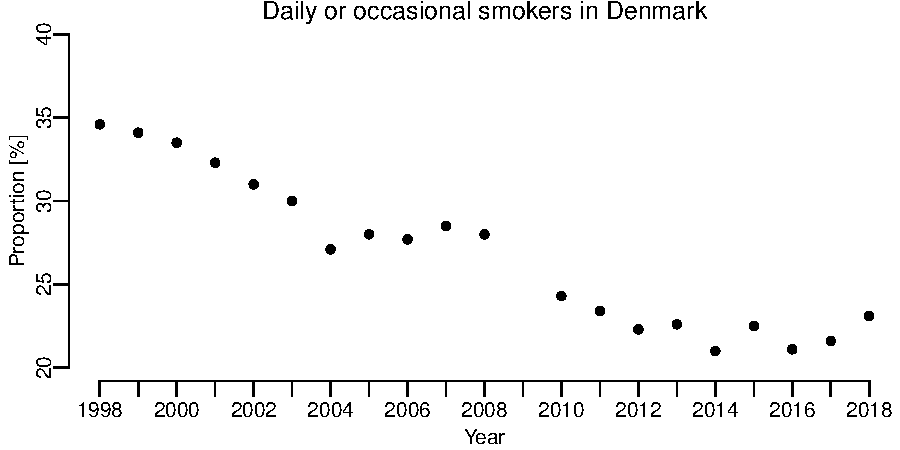
\includegraphics{rawDataPlot}
\caption{The proportion of daily or occasional smokers in Denmark during the last 20 years estimated from survey data and reported by the Danish Health Authority. The 2009 measurement is missing due to problems with representativeness.}
\label{fig:rawDataPlot}
\end{figure}

The concept of ``trend'' is not itself well-defined and it is often up
to each researcher to define exactly what is meant by ``trend'' (Esterby
1993). Consequently, it is not obvious, what constitutes a \emph{change}
in trend, and that makes it difficult to compare statistical methods to
detect trend changes, since they attempt to address slightly different
problems.

Change-point analysis is an often-used approach for detecting if a
change (of a prespecified type) has taken place (Basseville and
Nikiforov 1993; Barry and Hartigan 1993). However, change-point analysis
is marred by the fact that change-points that happen close to the
boundary of the observed time frame are notoriously difficult to detect,
and that they assume that change-points are abrupt changes that occur at
specific time point.

Another common approach to analyse trends in time series is to apply a
low-pass smoothing filter to the observed data in order to remove noise
and extract the underlying latent trend (Chandler and Scott 2011). But
in addition to the smoothing filter, it is also necessary to circumvent
the problem of what constitutes a change in trend so it is necessary to
specify a decision criterion to determine if any filtered changes are
relevant.

Gottlieb and Müller (2012) define a stickiness coefficient for
longitudinal data and use the stickiness coefficient to summarize the
extent to which deviations from the mean trajectory tend to co-vary over
time. While the stickiness coefficient determines changes from the
expected trend it is a measure that is not easily interpreted.

We propose a new method for evaluating changes in the latent trend,
\(f\), which starts by a clear specification of the problem and relevant
measures of the trend: The Trend Direction Index gives a local
probability of the monotonicity of \(f\) and provides an answer to the
research question ``What is the probability that the latent trend is
increasing?''. The Expected Trend Instability index gives the expected
number of changes in the monotonicity of \(f\) on an interval and
answers research questions about the rate of changes in direction of
\(f\) and can be used to evaluate the statement in the news paper that
,,It is the first time in 20 years that \(f\) has stopped decreasing and
started to increase''. Besides providing exact answers to specific and
relevant research questions, our proposed method estimates the actual
probability that the trend is changing.

The manuscript is structured as follows: In Section \ref{sec:method} we
present our statistical model based on a latent Gaussian process
formulation giving rise to analytic expressions for the Trend Direction
Index and the Expected Trend Instability index conditional on observed
data. Section \ref{sec:estimation} is concerned with estimating the
models parameters, and we give an extended application to the
development of the proportion of smokers in Denmark during the last 20
years in Section \ref{sec:application}. We conclude with a discussion.

Proofs of propositions are given in the supplmentary material, and
reproducible code and Stan implementations are available at the first
author's GitHub repository (Jensen 2019).

\section{Methods}\label{sec:method}

In the following we assume that reality evolves in continuous time
\(t \in \mathcal{T} \subset \mathbb{R}\) and that there exists a random,
latent function \(f = \left\{f(t) : t \in \mathcal{T}\right\}\)
sufficiently smooth on a compact subset of the real line,
\(\mathcal{T}\), that governs the underlying evolution of some
observable characteristic in a population. We can observe this latent
characteristic with noise by sampling \(f\) at discrete time points
according to the additive model \(Y_i = f(t_i) + \varepsilon_i\) where
\(\varepsilon_i\) is a zero mean random variable independent of
\(f(t_i)\). Given observations of the form \((Y_i, t_i)_{i=1}^n\) we are
interested in modeling the dynamical properties of \(f\).

The trend of \(f\) is defined as its instantaneous slope given by the
function \(df(t) = \left(\frac{\mathrm{d}f(s)}{\mathrm{d}s}\right)(t)\),
and \(f\) is increasing and has a positive trend at \(t\) if
\(df(t) > 0\), and \(f\) is decreasing with a negative trend at \(t\) if
\(df(t) < 0\). A change in trend is defined as a change in the sign of
\(df\), i.e., when \(f\) goes from increasing to decreasing or vice
versa. As \(f\) is a random function there are no exact points in time
where \(df\) changes sign. There is instead a gradual and continuous
change in the monotonicity of \(f\), and an assessment of a change in
trend is defined by the probability of the sign of \(df\). This stands
in contrast to traditional change-point models which assume that there
are one or more exact time points where a sudden change in function or
its parameterization occurs (Carlstein, Müller, and Siegmund 1994).

The probability that a trend is changing at time \(t\) is quantified by
the Trend Direction Index

\begin{align}
  \mathrm{TDI}(t, \delta) = P(df(t + \delta ) > 0 \mid \mathcal{F}_t), \quad t \in \mathcal{T}\label{eq:TCIdef}
\end{align}

where \(\mathcal{F}_t\) is a \(\sigma\)-algebra of available information
observed up until time \(t\). The value of \(\mathrm{TDI}(t, \delta)\)
is a local probabilistic index, and it is equal to the probability that
\(f\) is increasing at time \(t + \delta\) given everything known about
the data generating process up until and including time \(t\). A similar
definition can be given for a negative trend but that is equal to
\(1 - \mathrm{TDI}(t, \delta)\) and therefore redundant. The sign of
\(\delta\) determines whether the Trend Direction Index estimates the
past (\(\delta \leq 0\)) or forecasts the future (\(\delta > 0\)). Most
of the examples seen in the news concerning public health outcomes are
concerned with \(t\) being equal to the current calendar time and
\(\delta = 0\). This excludes the usage of both change-point and
segmented regression models (Quandt 1958) as there are no observations
available beyond the stipulated change-point. A useful
reparameterization of the Trend Direction Index is
\(\mathrm{TDI}(\max \mathcal{T}, t - \max \mathcal{T})\) with
\(t \leq \max \mathcal{T}\). This parameterization conditions on the
full observation period and looks back in time whereas setting
\(t = \max \mathcal{T}\) corresponds to the current Trend Direction
Index at the end of the observation period.

In addition to the Trend Direction Index we define a global measure of
trend instability. Informally, we say that a random function \(f\) is
\textit{trend stable} on an interval \(\mathcal{I}\) if its sample paths
maintain their monotonicity so that the trends do not change sign on the
interval. To quantify the trend \emph{in}stability we propose to use the
expected number of zero-crossings by \(df\) on \(\mathcal{I}\). We
define the Expected Trend Instability as

\begin{align}
  \text{ETI}(\mathcal{I}) = \E\left[\#\left\{t \in \mathcal{I} : df(t) = 0\right\} \mid \mathcal{F}\right]\label{eq:ETIdef}
\end{align}

equal to the expected value of the size of the random set of
zero-crossings by \(df\) on \(\mathcal{I}\) when conditioning on a
suitable \(\sigma\)-algebra \(\mathcal{F}\). A common case is when
\(\mathcal{F}\) is generated by all observed data on \(\mathcal{T}\) and
\(\mathcal{I} \subseteq \mathcal{T}\). The lower
\(\text{ETI}(\mathcal{I})\) is, the more stable is the trend of \(f\) on
\(\mathcal{I}\) and vice versa.

These two general definitions of trendiness will be evaluated in the
light of a particular statistical model in the next sections leading to
expressions of their estimates.

\subsection{Latent Gaussian Process
Model}\label{latent-gaussian-process-model}

The definitions in the previous section impose restrictions on the
latent function \(f\). We shall assume that \(f\) is a Gaussian process
on \(\mathcal{T}\). From a Bayesian perspective this is equivalent to
imposing an infinite dimensional prior distribution on the latent
characteristic that governs the observed outcomes. Statistical models
with Gaussian process priors are a flexible approach for non-parametric
regression (Radford 1999). Using a latent Gaussian process also provides
an analytically tractable way for performing statistical inference on
its derivatives. The general idea of our model is to apply the
properties of the Gaussian process prior on the latent characteristic to
update its the finite dimensional distributions by conditioning on the
observed data. This results in a posterior Gaussian process and its
derivatives from which estimates of the trendiness indices will be
derived.

A random function \(f\) is a Gaussian process if and only if the vector
\((f(t_1), \ldots, f(t_n))\) has a multivariate normal distribution for
every finite set of evaluation points \((t_1, \ldots, t_n)\), and we
write \(f \sim \mathcal{GP}(\mu(\cdot), C(\cdot, \cdot))\) where \(\mu\)
is the mean function and \(C\) is a symmetric, positive definite
covariance function (Cramer and Leadbetter 1967). We observed dependent
data in terms of outcomes and their associated sampling times,
\((Y_i, t_i)_{i=1}^n\), and we assume that the data are generated by the
hierarchical model

\begin{align}
\begin{split}
  f \mid \beta, \theta &\sim \mathcal{GP}(\mu_\beta(\cdot), C_\theta(\cdot,\cdot))\\
  Y_i \mid t_i, f(t_i), \Theta &\overset{iid}{\sim} N(f(t_i), \sigma^2), \quad \Theta = (\beta, \theta, \sigma)
\end{split}
\label{eq:generatingProcess}
\end{align}

where \(\beta\) is a vector of parameters for the mean function of
\(f\), \(\theta\) is a vector of parameters governing the covariance of
\(f\), and \(\sigma\) is the conditional standard deviation of the
observations.

\vspace{0.2cm}

\begin{assumption}
We assume the following regularity conditions.
\begin{enumerate}
  \item[A1:]{$f$ is a separable Gaussian process.}
  \item[A2:]{$\E[f(t) \mid \beta, \theta] = \mu_{\beta}(t)$ is a twice continuously differentiable function.}
  \item[A3:]{$\Cov[f(s), f(t) \mid \beta, \theta] = C_\theta(s,t)$ has mixed third-order partial derivatives continuous at the diagonal.}
  \item[A4:]{The joint distribution of $(df(t), d^2\!f(t) \mid \beta, \theta)$ is non-degenerate at any $t$ i.e., $\Cov[df(t), df(t) \mid \beta, \theta] > 0$ and $-1 < \Cor[df(t), d^2\!f(t) \mid \beta, \theta] < 1$.}
\end{enumerate}
\label{assumptions}
\end{assumption}

Under the above assumptions, an important property of a Gaussian process
is that it together with its first and second derivatives is a
multivariate Gaussian process with explicit expressions for the joint
mean, covariance and cross-covariance functions. Specifically, the joint
distribution of the latent function, \(f\), and its first and second
derivatives, \(df\) and \(d^2\!f\), is the multivariate Gaussian process

\begin{align}
  \begin{bmatrix}f(s)\\ df(t)\\ d^2\!f(u)\end{bmatrix} \mid \beta, \theta &\sim \mathcal{GP}\left(\begin{bmatrix}\mu_\beta(s)\\ d\mu_\beta(t)\\ d^2\!\mu_\beta(u)\end{bmatrix}, \begin{bmatrix}C_\theta(s, s^\prime) & \partial_2 C_\theta(s, t) & \partial_2^2 C_\theta(s, u)\\ \partial_1 C_\theta(t, s) & \partial_1 \partial_2 C_\theta(t, t^\prime) & \partial_1 \partial_2^2 C_\theta(t, u)\\ \partial_1^2 C_\theta(u, s) & \partial_1^2\partial_2 C_\theta(u, t) & \partial_1^2 \partial_2^2 C_\theta(u, u^\prime)\end{bmatrix}\right)\label{eq:latentJoint}
\end{align}

where \(d^k\!\mu_\beta\) is the \(k\)'th derivative of \(\mu_\beta\) and
\(\partial_j^k\) denotes the \(k\)'th order partial derivative with
respect to the \(j\)'th variable (Cramer and Leadbetter 1967).
Proposition \ref{prop:GPposterior} states the joint posterior
distribution of \((f, df, d^2\!f)\) conditional on the observed data.

\vspace{0.2cm}

\begin{proposition}
Let the data generating model be defined as in Equation (\ref{eq:generatingProcess}) and $\mathbf{Y} = (Y_1, \ldots, Y_n)$ the vector of observed outcomes together with its sampling times $\mathbf{t} = (t_1, \ldots, t_n)$. Then by the conditions in Assumption \ref{assumptions} the joint distribution of $(f, df, d^2\!f)$ conditional on $\mathbf{Y}$ and $\mathbf{t}$ evaluated at the vector $\mathbf{t}^\ast$ of $p$ time points is
\begin{align*}
\begin{bmatrix}f(\mathbf{t}^\ast)\\ df(\mathbf{t}^\ast)\\ d^2\!f(\mathbf{t}^\ast)\end{bmatrix} \mid \mathbf{Y}, \mathbf{t}, \Theta \sim N\left(\bm{\mu},  \bm{\Sigma}\right)
\end{align*}
where $\bm{\mu} \in \mathbb{R}^{3p}$ is the column vector of posterior expectations and $\bm{\Sigma} \in \mathbb{R}^{3p \times 3p}$ is the joint posterior covariance matrix. Partitioning these as
\begin{align*}
  \bm{\mu} = \begin{bmatrix}\mu_{f}(\mathbf{t^\ast} \mid \Theta)\\ \mu_{df}(\mathbf{t^\ast} \mid \Theta)\\ \mu_{d^2\!f}(\mathbf{t^\ast} \mid \Theta)\end{bmatrix}, \quad \bm{\Sigma} = \begin{bmatrix}\Sigma_{f}(\mathbf{t^\ast},\mathbf{t^\ast} \mid \Theta) &  \Sigma_{f,df}(\mathbf{t^\ast},\mathbf{t^\ast} \mid \Theta) & \Sigma_{f,d^2\!f}(\mathbf{t^\ast},\mathbf{t^\ast} \mid \Theta)\\  \Sigma_{f,df}(\mathbf{t^\ast},\mathbf{t^\ast} \mid \Theta)^T & \Sigma_{df}(\mathbf{t^\ast},\mathbf{t^\ast} \mid \Theta) & \Sigma_{df,d^2\!f}(\mathbf{t^\ast},\mathbf{t^\ast} \mid \Theta)\\ \Sigma_{f,d^2\!f}(\mathbf{t^\ast}, \mathbf{t^\ast} \mid \Theta)^T & \Sigma_{df,d^2\!f}(\mathbf{t^\ast}, \mathbf{t^\ast} \mid \Theta)^T & \Sigma_{d^2\!f}(\mathbf{t^\ast}, \mathbf{t^\ast} \mid \Theta)\end{bmatrix} 
\end{align*}
the individual components are given by
\begin{align*}
  \mu_{f}(\mathbf{t}^\ast \mid \Theta) &= \mu_\beta(\mathbf{t}^\ast) + C_\theta(\mathbf{t}^\ast, \mathbf{t})\left(C_\theta(\mathbf{t}, \mathbf{t}) + \sigma^2 I\right)^{-1}\left(\mathbf{Y} - \mu_\beta(\mathbf{t})\right)\\
  \mu_{df}(\mathbf{t}^\ast \mid \Theta) &= d\mu_\beta(\mathbf{t}^\ast) + \partial_1 C_\theta(\mathbf{t}^\ast, \mathbf{t})\left(C_\theta(\mathbf{t}, \mathbf{t}) + \sigma^2 I\right)^{-1}\left(\mathbf{Y} - \mu_\beta(\mathbf{t})\right) \\
  \mu_{d^2\!f}(\mathbf{t}^\ast \mid \Theta) &= d^2\!\mu_\beta(\mathbf{t}^\ast) + \partial_1^2 C_\theta(\mathbf{t}^\ast, \mathbf{t})\left(C_\theta(\mathbf{t}, \mathbf{t}) + \sigma^2 I\right)^{-1}\left(\mathbf{Y} - \mu_\beta(\mathbf{t})\right)\\
  \Sigma_{f}(\mathbf{t}^\ast, \mathbf{t}^\ast \mid \Theta) &= C_\theta(\mathbf{t}^\ast, \mathbf{t}^\ast) - C_\theta(\mathbf{t}^\ast, \mathbf{t})\left(C_\theta(\mathbf{t}, \mathbf{t}) + \sigma^2 I\right)^{-1} C_\theta(\mathbf{t}, \mathbf{t}^\ast)\\
  \Sigma_{df}(\mathbf{t}^\ast, \mathbf{t}^\ast \mid \Theta) &= \partial_1\partial_2C_\theta(\mathbf{t}^\ast, \mathbf{t}^\ast) - \partial_1C_\theta(\mathbf{t}^\ast, \mathbf{t})\left(C_\theta(\mathbf{t}, \mathbf{t}) + \sigma^2 I\right)^{-1} \partial_2C_\theta(\mathbf{t}, \mathbf{t}^\ast)\\
  \Sigma_{d^2\!f}(\mathbf{t}^\ast, \mathbf{t}^\ast \mid \Theta) &= \partial_1^2\partial_2^2 C_\theta(\mathbf{t}^\ast, \mathbf{t}^\ast) - \partial_1^2 C_\theta(\mathbf{t}^\ast, \mathbf{t})\left(C_\theta(\mathbf{t}, \mathbf{t}) + \sigma^2 I\right)^{-1} \partial_2^2 C_\theta(\mathbf{t}, \mathbf{t}^\ast)\\
  \Sigma_{f, df}(\mathbf{t}^\ast, \mathbf{t}^\ast \mid \Theta) &= \partial_2 C_\theta(\mathbf{t}^\ast, \mathbf{t}^\ast) - C_\theta(\mathbf{t}^\ast, \mathbf{t})\left(C_\theta(\mathbf{t}, \mathbf{t}) + \sigma^2 I\right)^{-1} \partial_2 C_\theta(\mathbf{t}, \mathbf{t}^\ast)\\
  \Sigma_{f, d^2\!f}(\mathbf{t}^\ast, \mathbf{t}^\ast \mid \Theta) &= \partial_2^2 C_\theta(\mathbf{t}^\ast, \mathbf{t}^\ast) - C_\theta(\mathbf{t}^\ast, \mathbf{t})\left(C_\theta(\mathbf{t}, \mathbf{t}) + \sigma^2 I\right)^{-1} \partial_2^2 C_\theta(\mathbf{t}, \mathbf{t}^\ast)\\
  \Sigma_{df, d^2\!f}(\mathbf{t}^\ast, \mathbf{t}^\ast \mid \Theta) &= \partial_1 \partial_2^2 C_\theta(\mathbf{t}^\ast, \mathbf{t}^\ast) - \partial_1 C_\theta(\mathbf{t}^\ast, \mathbf{t})\left(C_\theta(\mathbf{t}, \mathbf{t}) + \sigma^2 I\right)^{-1} \partial_2^2 C_\theta(\mathbf{t}, \mathbf{t}^\ast)
\end{align*}
\label{prop:GPposterior}
\end{proposition}

Proposition \ref{prop:GPposterior} grants the foundation for the rest of
the methodological development. In the following two subsection we show
how the Trend Direction Index and the Expected Trend Instability can be
expressed under the data generating model in Equation
(\ref{eq:generatingProcess}) using the results of Proposition
\ref{prop:GPposterior}.

\subsection{The Trend Direction Index}\label{the-trend-direction-index}

The Trend Direction Index was defined generally in Equation
(\ref{eq:TCIdef}). Conditioning on the \(\sigma\)-algebra of all
observed data we may express the Trend Direction Index under the model
in Equation (\ref{eq:generatingProcess}) through the posterior
distribution of \(df\). The following proposition states this result.

\vspace{0.2cm}

\begin{proposition}
Let $\mathcal{F}_t$ be the $\sigma$-algebra generated by $(\mathbf{Y}, \mathbf{t})$ where $\mathbf{Y} = (Y_1, \ldots, Y_n)$ is the vector of observed outcomes and $\mathbf{t} = (t_1, \ldots, t_n)$ the associated sampling times. Furthermore, assume that assumptions A1-A3 above are fulfilled. The Trend Direction Index defined in Equation (\ref{eq:TCIdef}) can then be written in terms of the posterior distribution of $df$ as
\begin{align*}
  \mathrm{TDI}(t, \delta \mid \Theta) &= P(df(t + \delta ) > 0 \mid \mathbf{Y}, \mathbf{t}, \Theta)\\
  &= \frac{1}{2} + \frac{1}{2}\Erf\left(\frac{\mu_{df}(t + \delta \mid \Theta)}{2^{1/2}\Sigma_{df}(t + \delta, t + \delta \mid \Theta)^{1/2}}\right)
\end{align*}
where $\Erf\colon\, x \mapsto 2\pi^{-1/2}\int_0^x \exp(-u^2)\mathrm{d}u$ is the error function and $\mu_{df}$ and $\Sigma_{df}$ are the posterior mean and covariance of the trend defined in Proposition \ref{prop:GPposterior}.
\label{prop:TDIposterior}
\end{proposition}

Proposition \ref{prop:TDIposterior} shows that the Trend Direction Index
is equal to \(0.5\) when \(\mu_{df}(t + \delta \mid \Theta) = 0\)
corresponding to when the expected value of the posterior of \(f\) is
locally constant at time \(t + \delta\). A decision rule based on
\(\mathrm{TDI}(t, \delta \mid \Theta) \lessgtr 50\%\) is therefore a
natural choice for assessing the local trendiness of \(f\). However,
different thresholds based on external loss or utility functions can be
used depending on the application. Note that the requirements of
assumptions A2 and A3 can be reduced to first order differentiable (A2)
and mixed second derivatives (A3), respectively, if only the TDI is to
be used.

\begin{figure}[htb]
\center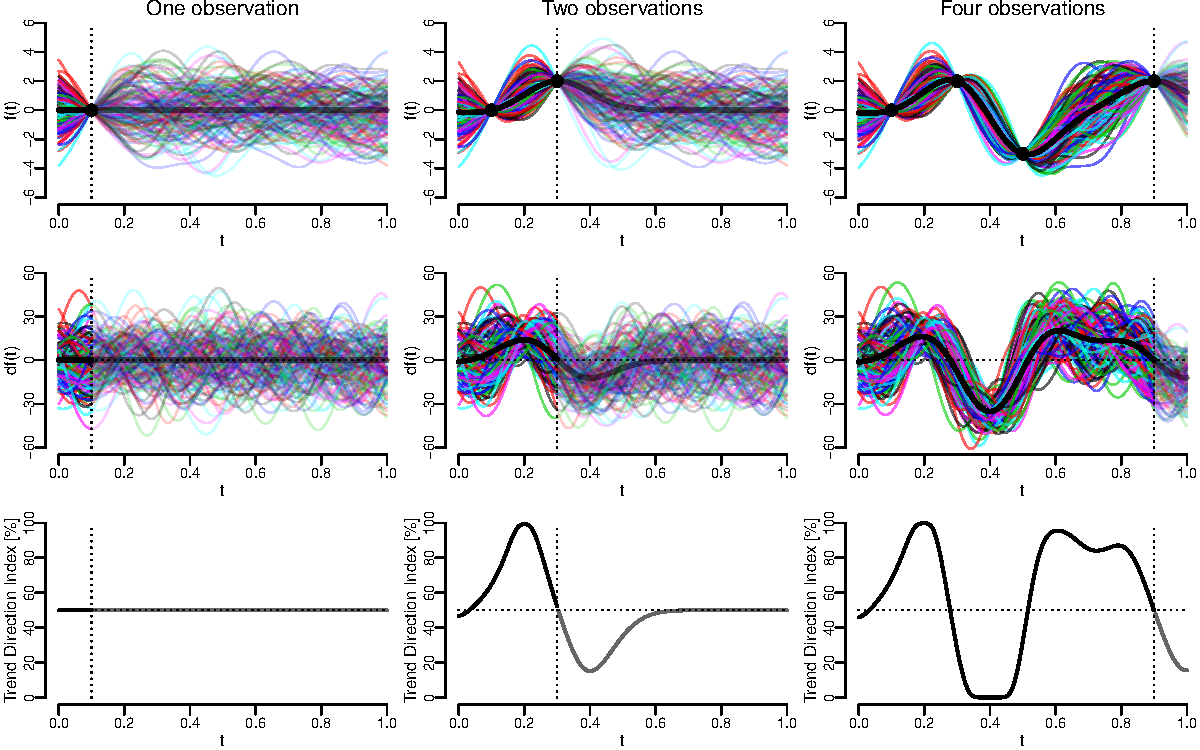
\includegraphics{TDIexample}
\caption{150 realizations from the posterior distribution of $f$ (top row), $df$ (middle row) with expected values in bold and the Trend Direction Index (bottom row) conditional on one, two and four noise free observations. Dotted vertical lines show the points in time after which forecasting takes place.}
\label{fig:probabilisticExample}
\end{figure}

The Trend Direction Index is illustrated in Figure
\ref{fig:probabilisticExample} in the noise free case, \(\sigma = 0\),
with known values of \(\beta\) and \(\theta\), and where the prior
expected value of \(f\) is set equal to \(\mu_{\beta}(t) = 0\). The
first and second rows of the plot show 150 random sample paths from the
posterior distribution of \((f, df)\) with the posterior expectations in
bold lines, and the third row shows the Trend Direction Index. Since the
parameters, \(\Theta\), of \(f\) are known in this example, the Trend
Direction Index is a deterministic function of time. The three columns
in the plot show how the posterior of \(f\), \(df\), and the
\(\mathrm{TDI}\) are updated after one, two and four observations both
forwards and backwards in time. The figure shows how the inclusion of
additional observations results in changes of the posterior distribution
of the trend and the Trend Direction Index. The variation of the
forecasts remains unchanged, whereas the posterior distribution back in
time restricts the variation of the curves to accommodate the
observations. The vertical dotted lines denote the point in time after
which forecasting occurs. When forecasting beyond the last observation,
the posterior of \(f\) becomes more and more dominated by its prior
implying that \(df\) becomes symmetric around zero so that the Trend
Direction Index stabilizes around \(50\%\).

\subsection{The Expected Trend
Instability}\label{the-expected-trend-instability}

The Expected Trend Instability was defined in Equation (\ref{eq:ETIdef})
as the expected number of roots of the trend on an interval conditional
on observed data. Now we make this concept more precise and frame it in
the context of the latent Gaussian process model. Let \(\mathcal{I}\) be
a compact subset of the real line and consider the random càdlàg
function

\begin{align*}
  N_\mathcal{I}(t) = \#\left\{s \leq t : df(s) = 0, s \in \mathcal{I}\right\}
\end{align*}

counting the cumulative number of points in \(\mathcal{I}\) up to time
\(t\) where the trend is equal to zero. The Expected Trend Instability
on \(\mathcal{I}\) is equal to

\begin{align*}
  \mathrm{ETI}(\mathcal{I} \mid \Theta) = \E\left[N_{\mathcal{I}}\left(\max \mathcal{I}\right) \mid \Theta, \mathcal{F}\right]
\end{align*}

giving the expected total number of zero-crossings by \(df\) on
\(\mathcal{I}\). The following proposition gives the expression for the
Expected Trend Instability under the data generating model in Equation
(\ref{eq:generatingProcess}).

\vspace{0.2cm}

\begin{proposition}
Let $\mathcal{F}$ be the $\sigma$-algebra generated by the observed data $(\mathbf{Y}, \mathbf{t})$ and $\mu_{df}$, $\mu_{d^2\!f}$, $\Sigma_{df}$, $\Sigma_{d^2\!f}$ and $\Sigma_{df,d^2\!f}$ the moments of the joint posterior distribution of $(df, d^2\!f)$ as stated in Proposition \ref{prop:GPposterior}, and assume that all assumptions A1-A4 are fulfilled. The Expected Trend Instability is then
\begin{align*}
  \mathrm{ETI}(\mathcal{I} \mid \Theta) = \int_{\mathcal{I}} d\mathrm{ETI}(t \mid \Theta)\mathrm{d}t
\end{align*}
where $d\mathrm{ETI}$ is the local Expected Trend Instability given by
\begin{align*}
d\mathrm{ETI}(t, \mathcal{T} \mid \Theta) = \lambda(t \mid \Theta)\phi\left(\frac{\mu_{df}(t \mid \Theta)}{\Sigma_{df}(t,t \mid \Theta)^{1/2}}\right)\left(2\phi(\zeta(t\mid \Theta)) + \zeta(t\mid \Theta)\Erf\left(\frac{\zeta(t\mid \Theta)}{2^{1/2}}\right)\right)
\end{align*}
and $\phi\colon\, x \mapsto 2^{-1/2}\pi^{-1/2}\exp(-\frac{1}{2}x^2)$ is the standard normal density function, $\Erf\colon\, x \mapsto 2\pi^{-1/2}\int_0^x \exp(-u^2)\mathrm{d}u$ is the error function, and $\lambda$, $\omega$ and $\zeta$ are functions defined as
\begin{align*}
  \lambda(t \mid \Theta) &= \frac{\Sigma_{d^2\!f}(t,t \mid \Theta)^{1/2}}{\Sigma_{df}(t,t \mid \Theta)^{1/2}}\left(1-\omega(t \mid \Theta)^2\right)^{1/2}\\
  \omega(t \mid \Theta) &= \frac{\Sigma_{df,d^2\!f}(t,t \mid \Theta)}{\Sigma_{df}(t,t \mid \Theta)^{1/2}\Sigma_{d^2\!f}(t,t \mid \Theta)^{1/2}}\\
  \zeta(t\mid \Theta) &= \frac{\mu_{df}(t\mid \Theta)\Sigma_{d^2\!f}(t,t\mid \Theta)^{1/2}\omega(t)\Sigma_{df}(t,t\mid \Theta)^{-1/2} - \mu_{d^2\!f}(t\mid \Theta)}{\Sigma_{d^2\!f}(t,t\mid \Theta)^{1/2}\left(1 - \omega(t\mid \Theta)^2\right)^{1/2}}
\end{align*}
\label{prop:ETIposterior}
\end{proposition}

To illustrate the Expected Trend Instability, Figure
\ref{fig:ETIexample} shows \(25\) random Gaussian processes on the unit
interval simulated under three different values of \(\mathrm{ETI}\). The
sample paths are paired so that each function in the first row has an
associated trend function in the second row. The different values of
\(\mathrm{ETI}\) are set to \(0.25\), \(0.5\) and \(1\) corresponding to
the expected number of times that the functions change monotonicity or
equivalently that the trend crosses zero on that interval. Sample paths
that are \textit{trend stable}, i.e., always increasing/decreasing, are
shown by solid blue lines, and sample paths that are
\textit{trend unstable}, i.e., the derivatives crosses zero, are shown
by dashed gold colored lines. It is seen that for low values of
\(\mathrm{ETI}\) most of the sample paths preserve their monotonicity on
the interval and their associated derivatives are correspondingly either
always positive or negative. For larger values of \(\mathrm{ETI}\), more
of the trends start crossing zero implying less stability in the
monotonicity of \(f\). We note that even though we are only modeling a
single curve, the Expected Trend Instability is defined in terms of a
posterior distribution of random curves which is what the figure
illustrates.

\begin{figure}[htb]
\center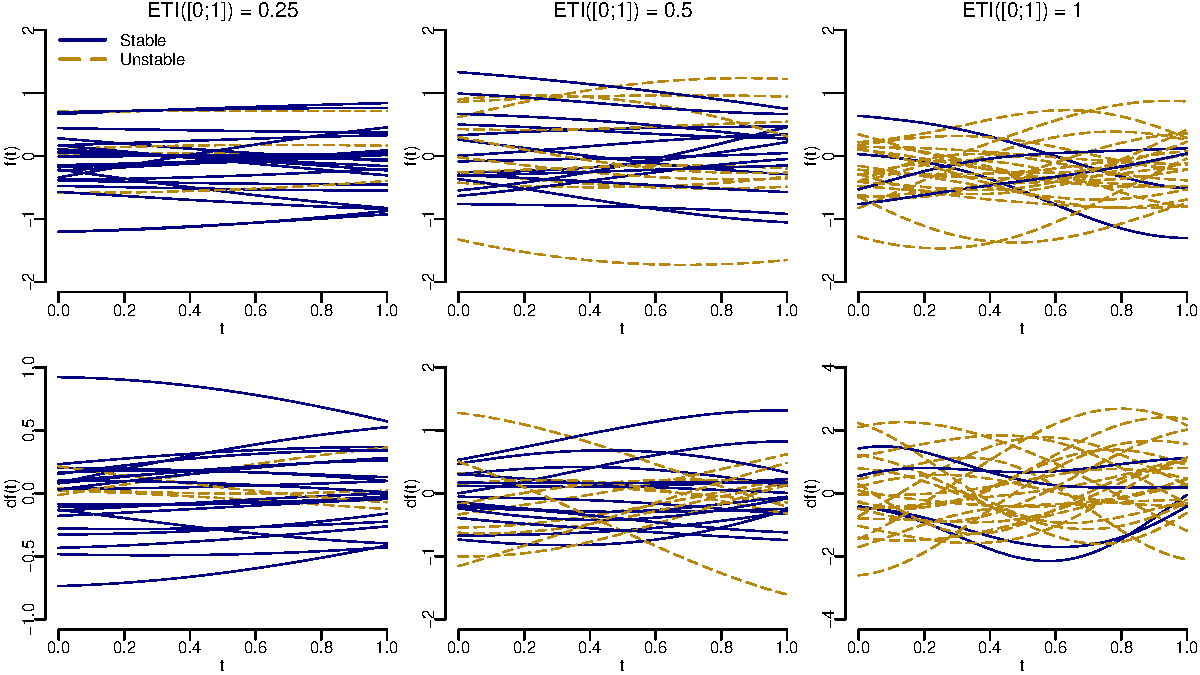
\includegraphics{ETIexample}
\caption{$25$ random pairs sampled from the joint distribution of a Gaussian Process ($f$) and its derivative ($df$) with different values of Expected Trend Instability (ETI). The first row shows samples from $f$, and the second row shows samples from $df$. The columns define different values of ETI. Sample paths that are trend stable are shown by solid blue lines, and unstable sample paths are shown by dashed gold colored lines.}
\label{fig:ETIexample}
\end{figure}

\section{Estimation}\label{sec:estimation}

The trendiness indices depend on the parameters \(\Theta\) of the latent
Gaussian process. These parameters must be estimated from the observed
data, and we consider two different estimation procedures: maximum
likelihood (also called Empirical Bayes) estimation and a fully Bayesian
estimator.

The maximum likelihood estimator consists of finding the values of the
parameters that maximize the marginal likelihood of the observed data
and plugging these into the expressions of the posterior distributions
and the trendiness indices. The marginal distribution of \(\mathbf{Y}\)
is found by integrating out the distribution of the latent Gaussian
process in the conditional observation model
\(\mathbf{Y} \mid f(\mathbf{t}), \mathbf{t}, \Theta\) in Equation
(\ref{eq:generatingProcess}). Since the observation model consists of
normal distributed random variables conditional on the latent Gaussian
process, the marginal distribution is multivariate normal with
expectation \(\mu_\beta(\mathbf{t})\) and \(n \times n\) covariance
matrix \(C_\theta(\mathbf{t}, \mathbf{t}) + \sigma^2 I\). The marginal
log likelihood function is therefore

\begin{align}
\log L(\Theta \mid \mathbf{Y}, \mathbf{t}) &\propto - \frac{1}{2}\log |C_{\theta}(\mathbf{t}, \mathbf{t}) + \sigma^2 I| - \frac{1}{2}(\mathbf{Y} - \mu_\beta(\mathbf{t}))^T\left[C_{\theta}(\mathbf{t}, \mathbf{t}) + \sigma^2 I\right]^{-1}(\mathbf{Y} - \mu_\beta(\mathbf{t}))\label{eq:margloglik}
\end{align}

and the maximum likelihood estimate
\(\widehat{\Theta^\text{ML}} = \argsup_{\Theta = (\beta, \theta, \sigma)} \log L(\Theta \mid \mathbf{Y}, \mathbf{t})\)
can be obtained by numerical optimization or found as the roots to the
score equations
\(\nabla_\theta \log L(\Theta \mid \mathbf{Y}, \mathbf{t}) = 0\). This
estimate can then be plugged in to the expressions for the posterior
distributions of \((f, df, d^2\!f)\) in Proposition
\ref{prop:GPposterior} enabling simulation of the posterior
distributions at any vector of time points. Point estimates of the Trend
Direction Index and the Expected Trend Instability are then
\(\mathrm{TDI}(t, \delta \mid \widehat{\Theta^\text{ML}})\) and
\(\mathrm{ETI}(\mathcal{I} \mid \widehat{\Theta^\text{ML}})\) according
to Propositions \ref{prop:TDIposterior} and \ref{prop:ETIposterior}
respectively.

The maximum likelihood estimator is easy to implement and fast to
compute, but it is difficult to propagate the uncertainties of the
parameter estimates through to the posterior distributions and the
trendiness indices. This is disadvantageous since in order to conduct a
qualified assessment of trendiness we are not only interested in point
estimates but also the associated uncertainties. A Bayesian estimator,
while slower to compute, facilitates a straightforward way to encompass
all uncertainties in the final estimates. To specify a Bayesian
estimator we must augment the data generating model in Equation
(\ref{eq:generatingProcess}) with another hierarchical level specifying
a prior distribution of the model parameters. We therefore add the
following level

\begin{align*}
  (\beta, \theta, \sigma) \sim G(\Theta \mid \Psi, \mathbf{t})
\end{align*}

to the specification where \(G\) is some family of distribution
functions indexed by a vector of hyper-parameters \(\Psi\). The joint
distribution of the model can be factorized as

\begin{align*}
  P(\mathbf{Y}, f(\mathbf{t}), \Theta \mid \Psi, \mathbf{t}) = P(\mathbf{Y} \mid f(\mathbf{t}), \Theta, \Psi, \mathbf{t})P(f(\mathbf{t}) \mid \Theta, \Psi, \mathbf{t})G(\Theta \mid \Psi, \mathbf{t})
\end{align*}

and each conditional probability is specified by a sub-model in the
augmented hierarchy. We always condition on \(\Psi\) and \(\mathbf{t}\)
as they are considered fixed data. The posterior distribution of
\(\Theta\) given the observed outcomes is then

\begin{align*}
  P(\Theta \mid \mathbf{Y}, \Psi, \mathbf{t}) & = \frac{G(\Theta \mid \Psi, \mathbf{t})P(\mathbf{Y} \mid \Theta, \Psi, \mathbf{t})}{P(\mathbf{Y} \mid \Psi, \mathbf{t})}\\
   &= \frac{G(\Theta \mid \Psi, \mathbf{t}) \int P(\mathbf{Y} \mid f(\mathbf{t}), \Theta, \Psi, \mathbf{t})dP(f(\mathbf{t}) \mid \Theta, \Psi, \mathbf{t})}{\iint P(\mathbf{Y} \mid f(\mathbf{t}), \Theta, \Psi, \mathbf{t})dP(f(\mathbf{t}) \mid \Theta, \Psi, \mathbf{t})dG(\Theta \mid \Psi, \mathbf{t})}
\end{align*}

Let
\(\widetilde{\Theta} \sim P(\Theta \mid \mathbf{Y}, \Psi, \mathbf{t})\).
The posterior distribution of \(\Theta\) induces corresponding
distributions over the trendiness indices according to
\(\mathrm{TDI}(t, \delta \mid \widetilde{\Theta})\),
\(d\mathrm{EDI}(t, \mathcal{T}, \mid \widetilde{\Theta})\) and
\(\mathrm{EDI}(\mathcal{I} \mid \widetilde{\Theta})\). For example, the
Trend Direction Index in the Bayesian formulation is a surface in
\((t, \delta)\) where each value is a distribution over probability
values. We suggest to summarize the trendiness indices by their
posterior quantiles. For example, for the Trend Direction Index we
summarize its posterior distribution by functions \(Q_\tau\) such that

\begin{align*}
  P\left(\mathrm{TDI}\left(t, \delta \mid \widetilde{\Theta}\right) \leq \tau\right) = Q_\tau(t, \delta)
\end{align*}

with for example \(\tau \in \left\{0.025, 0.5, 0.975\right\}\) to obtain
95\% credibility intervals.

We have implemented both the maximum likelihood and the Bayesian
estimator in Stan (Carpenter et al. 2017) and R (R Core Team 2018) in
combination with the \texttt{rstan} package (Stan Development Team
2018). Stan is a probabilistic programming language enabling full
Bayesian inference using Markov chain Monte Carlo sampling. The Stan
implementation of the maximum likelihood estimator requires the marginal
maximum likelihood estimates of the parameters supplied as data, and
from these it will simulate random functions from the posterior
distribution of \((f, df, d^2\!f)\) on a user-supplied grid of time
points as well as return point estimates of \(\mathrm{TDI}\) and
\(d\mathrm{ETI}\). The latter can then be integrated numerically to
obtain the Expected Trend Instability on an interval. The Bayesian
estimator requires values of the hyper-parameters \(\Psi\) supplied as
data and from these it will generate random samples
\((\widetilde{\Theta}_1, \ldots, \widetilde{\Theta}_K)\) from
\(P(\Theta \mid \mathbf{Y}, \Psi, \mathbf{t})\) by Markov chain Monte
Carlo. These samples are then used to approximate the posterior
distribution of the Trend Direction Index by
\((\mathrm{TDI}(t, \delta \mid \widetilde{\Theta}_1), \ldots, \mathrm{TDI}(t, \delta \mid \widetilde{\Theta}_K))\)
and similarly for \(d\mathrm{ETI}\).

\section{Application: trend of proportion of Danish
smokers}\label{sec:application}

A report published by The Danish Health Authority in January 2019
updated the estimated proportion of daily or occasional smokers in
Denmark with new data from 2018 (The Danish Health Authority 2019). The
data was based on an online survey including 5017 participants. The
report also included data on the proportion of smokers in Denmark during
the last 20 years which was shown in Figure \ref{fig:rawDataPlot}. The
report was picked up by several news papers under headlines stating that
the proportion of smokers in Denmark had significantly increased for the
first time in two decades (Navne, Schmidt, and Rasmussen 2019). The
report published no statistical analyses for this statement but wrote,
that because the study population is so large, then more or less all
differences become statistically significant at the \(5\%\) level (this
was written as a \(95\%\) significance level in the report).

This data set provides an instrumental way of exemplifying our two
proposed measures of trendiness. In this application we wish to assess
the statistical properties of following questions:

\begin{itemize}
\item[Q1:]{Is the proportion of smokers increasing in the year 2018 conditional on data from the last 20 years?}
\item[Q2:]{If the proportion of smokers is currently increasing, when did this increase probably start?}
\item[Q3:]{Is it the first time during the last 20 years that the trend in the proportion of smokers has changed?}
\end{itemize}

A naive approach for trying to answer questions Q1 and Q2 is to apply
sequential \(\chi^2\)-tests in a \(2\times 2\) table. Table
\ref{tab:chisqtests} shows the p-values for the \(\chi^2\)-test of
independence between the proportion of smokers in 2018 and each of the
five previous years. Using a significance level of \(5\%\) the
conclusion is ambiguous. Compared to the previous year, there was no
significant change in the proportion in 2018. Three out of these five
comparisons fail to show a significant change in proportions. It is
therefore evident that such point-wise testing is not sufficiently
perceptive to catch the underlying continuous development.

\begin{table}[htbp]
\center
\begin{tabular}{c|rrrrr}
2018 & 2017 & 2016 & 2015 & 2014 & 2013\\ \hline
p-value & 0.074 & \textbf{0.020} & 0.495 & \textbf{0.012} & 0.576
\end{tabular}
\caption{p-values obtained from $\chi^2$-tests of independence between the proportion of smokers in 2018 and the five previous years. Numbers in bold are statistically significant differences at the $5\%$ level.}
\label{tab:chisqtests}
\end{table}

Similarly, a simple approach for trying to answer question Q3 would be
to look at the cumulative number of times that the difference in
proportion between consecutive years changes sign. In the data set there
were nine changes in the sign of the difference between the proportion
in each year and the proportion in the previous year giving this very
crude estimate of the number of times that the trend has changed. This
approach suffers from the facts that it is based on a finite difference
approximation at the sampling points to the continuous derivative, and
that it uses the noisy measurements instead the latent function.
Consequently, the changes in trend are quite unstable.

We now present an analysis of the data set using our method. To complete
the model specification in Equation (\ref{eq:generatingProcess}) we must
decide on the functional forms of the mean and covariance functions of
the latent Gaussian process. We considered three different mean
functions: a constant mean: \(\mu_\beta(t) = \beta_0\), a linear mean:
\(\mu_\beta(t) = \beta_0 + \beta_1 t\), and a quadratic mean:
\(\mu_\beta(t) = \beta_0 + \beta_1 t + \beta_2 t^2\). We considered the
Squared Exponential (SE), the Rational Quadratic (RQ), the Matern 3/2
(M3/2), and the Matern 5/2 (M5/2) covariance functions (C. E. Rasmussen
and Williams 2006). These covariance functions are

\begin{align}
\begin{split}
  C_\theta^\text{SE}(s, t) &= \alpha^2\exp\left(-\frac{(s-t)^2}{2\rho^2}\right), \quad \theta = (\alpha, \rho) > 0\\ 
  C_\theta^\text{RQ}(s, t) &= \alpha^2\left(1 + \frac{(s-t)^2}{2\rho^2\nu}\right)^{-\nu}, \quad \theta = (\alpha, \rho, \nu) > 0\\
  C_\theta^\text{M3/2}(s, t) &= \alpha^2\left(1 + \frac{\sqrt{3}\sqrt{(s-t)^2}}{\rho}\right)\exp\left(-\frac{\sqrt{3}\sqrt{(s-t)^2}}{\rho}\right), \quad \theta = (\alpha, \rho) > 0\\
  C_\theta^\text{M5/2}(s, t) &= \alpha^2\left(1 + \frac{\sqrt{5}\sqrt{(s-t)^2}}{\rho} + \frac{5(s-t)^2}{3\rho^2}\right)\exp\left(-\frac{\sqrt{5}\sqrt{(s-t)^2}}{\rho}\right), \quad \theta = (\alpha, \rho)  > 0
\end{split}
\label{eq:covariancefunctions}
\end{align}

We note that the Rational Quadratic covariance function converges on
\(\mathcal{T} \times \mathcal{T}\) to the Squared Exponential covariance
function for \(\nu \rightarrow \infty\). Note also that M3/2 is valid
for TDI but not for ETI since M3/2 does not fulfill the requirement of
mixed third-order partial derivatives of assumption A3.

The total combination of mean and covariance functions results in 12
candidate models, and to select the model providing the best fit to data
we used leave-one-out cross-validation based on maximum likelihood
estimation. For each model, \(\mathcal{M}\), we turn by turn excluded
data from a single year, and we let the leave-one-out data be denoted
\((\mathbf{Y}_{-i}, \mathbf{t}_{-i})\). Based on the leave-one-out data
sets we estimated the parameters
\(\Theta_{-i}^{\mathcal{M}} = (\beta, \theta, \sigma^2)\) for each model
by maximizing the marginal log-likelihood. These estimates are given by

\begin{align*}
\widehat{\Theta}_{-i}^\mathcal{M} = \argsup_{\Theta} \log L(\Theta \mid \mathbf{Y}_{-i}, \mathbf{t}_{-i}) 
\end{align*}

where the log likelihood function is given in Equation
(\ref{eq:margloglik}). These estimates were then plugged into the
expression for the posterior expectation of \(f\) in Proposition
\ref{prop:GPposterior} to obtain the leave-one-out predictions at times
\(t_i\). The mean squared error of prediction was calculated as the
squared errors between the leave-one-out predictions and the observed
values averaged across all data points

\begin{align*}
  \text{MSPE}_{\text{LOO}}^\mathcal{M} = \frac{1}{n}\sum_{i=1}^{n} \left(Y_i - \E[f(t_i) \mid \mathbf{Y}_{-i}, \mathbf{t}_{-i}, \widehat{\Theta}_{-i}^\mathcal{M}]\right)^2
\end{align*}

and the model providing the best fit to data was selected as
\(\mathcal{M}_{\text{opt}} = \argmin_\mathcal{M} \text{MSPE}_{\text{LOO}}^\mathcal{M}\).

\begin{table}[htbp]
\center
\begin{tabular}{l|rrrr}
 & SE & RQ & Matern 3/2 & Matern 5/2\\ \hline
Constant & 0.682 & \textbf{0.651} & 0.687 & 0.660\\
Linear & 0.806 & $\Leftarrow    $ & 0.896 & 0.865\\
Quadratic & 0.736 & $\Leftarrow$ & 0.800 & 0.785
\end{tabular}
\caption{Leave-one-out cross-validated mean squared error of prediction for each of the 12 candidate models. $\Leftarrow$ indicates numerical convergence to the SE covariance function.}
\label{tab:looTale}
\end{table}

Table \ref{tab:looTale} shows the mean squared error of prediction for
each candidate model. For the models with a Rational Quadratic
covariance function and a linear and a quadratic mean function the
parameter \(\nu\) diverged numerically implying convergence to the
Squared Exponential covariance function. Comparing the leave-one-out
mean squared error of prediction, the prior distribution of \(f\) in the
optimal model has a constant mean function and a Rational Quadratic
covariance function. The marginal maximum likelihood estimates of the
parameters in the optimal model were

\begin{align}
  \widehat{\beta_0^\text{ML}} = 28.001, \quad \widehat{\alpha^\text{ML}} = 4.543, \quad \widehat{\rho^\text{ML}} = 4.438, \quad \widehat{\nu^\text{ML}} = 1.020, \quad \widehat{\sigma^\text{ML}} = 0.622\label{eq:mlEstimates}
\end{align}

Figure \ref{fig:likFitPlot} shows the fit of the model by the maximum
likelihood method. The plots were obtained by plugging the maximum
likelihood estimates into the expressions for the posterior
distributions of \(f\) and \(df\) defined in Proposition
\ref{prop:GPposterior}, the Trend Direction Index in Proposition
\ref{prop:TDIposterior}, and the Expected Trend Instability in
Proposition \ref{prop:ETIposterior}. The predictions were performed on
an equidistant grid of \(500\) time points spanning the 20 years. The
plot of the posterior trend (top right) shows two regions in time where
the posterior mean of the derivative is positive, one around
\([2004; 2008]\) and one shortly after \(2015\) and until the end of the
observation period. The Trend Direction Index (bottom left) quantifies
this positive trendiness as a probability standing in \(2018\) and
looking back in time while also taking the uncertainty into account. The
bottom right panel shows the local Expected Trend Instability and its
integral is to the expected number of times that the trend has changed
sign. Table \ref{tab:summaries} summarizes the maximum likelihood
estimates of the Trend Direction Index at the end of the observation
period and the previous five years as well as the Expected Trend
Instability during the full observation period and during only the last
ten years. \(\text{Crosspoint}\) is the first point in time during the
last ten years where the Trend Direction Index became greater than
\(50\%\) i.e.,

\begin{align*}
\text{Crosspoint} = \argmin_{t \in [-10; 0]} \left\{2018 + t : \text{TDI}(2018, 2018 - t) \geq 50\%\right\}
\end{align*}

Based on the results from the maximum likelihood analysis we may answer
the questions by stating that the proportion of smokers in Denmark is
currently increasing with a probability of \(95.24\%\). This is,
however, not a recent development as the probability of an increasing
proportion has been greater than \(50\%\) since the middle of 2015. This
can be compared to the sequential \(\chi^2\)-tests in Table
\ref{tab:chisqtests}, which gave a cruder and less consistent result.
The estimated values of \(\mathrm{ETI}\) in Table \ref{tab:summaries}
show that there has been an average of \(3.68\) changes in the
monotonicity of the proportion during the last 20 years. This value does
support the statement by the news outlets that it is the first time in
20 years that the trend has changed. The value, however, reduces to 1.39
when only looking 10 years back, which is slightly less than half the
ETI for the longer period.

\begin{figure}[htb]
\center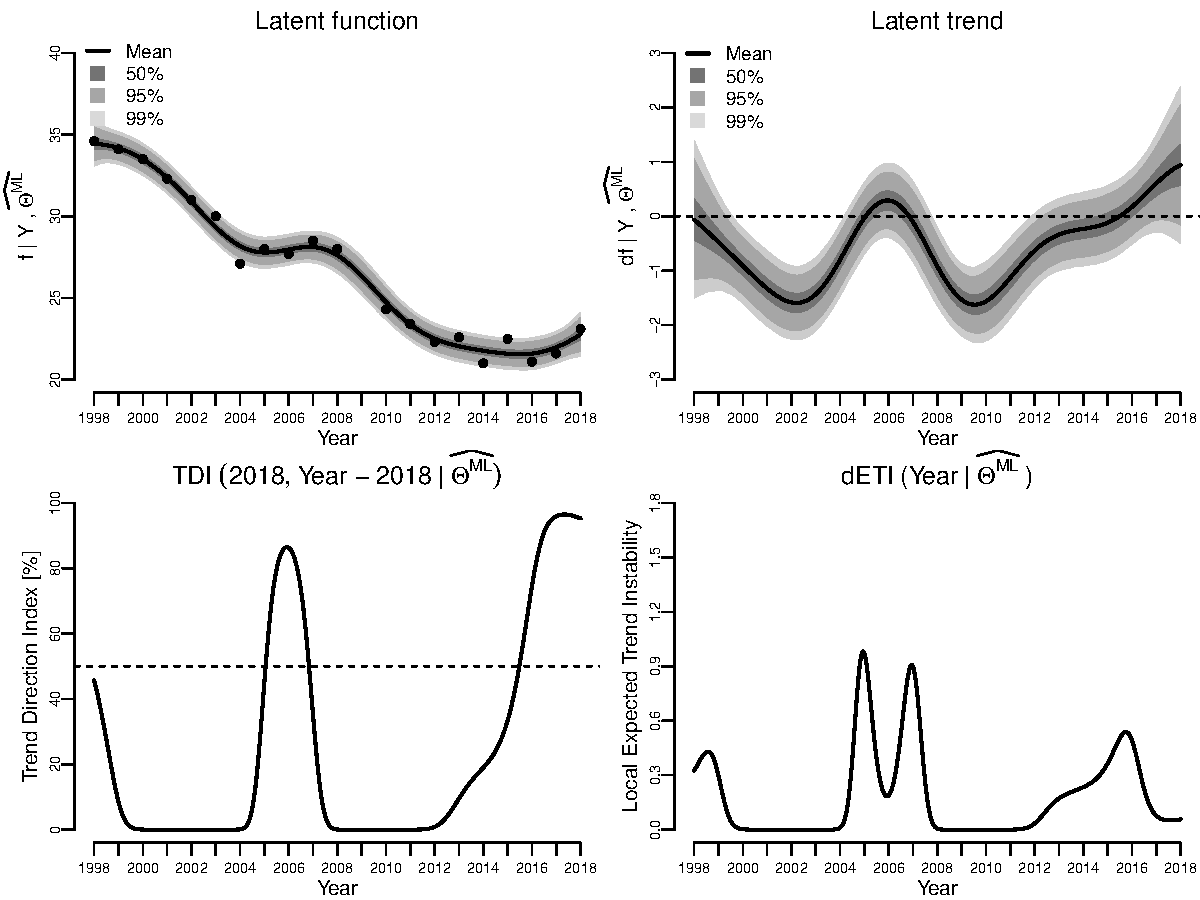
\includegraphics{likFitPlot}
\caption{Results from fitting the latent Gaussian process model by maximum likelihood. The first row shows the posterior distributions of $f$ (left) and $df$ (right) with the posterior means in bold and gray areas showing point-wise probability intervals for the posterior distribution. The second row shows the estimated Trend Direction Index (left) and the local Expected Trend Instability (right).}
\label{fig:likFitPlot}
\end{figure}

We also applied the Bayesian estimator to the data using the same prior
mean and covariance structure. The Bayesian estimator requires a prior
distribution for the model parameters. We used independent priors of the
form

\begin{align*}
G(\Theta \mid \Psi, \mathbf{t}) = G(\beta_0 \mid \Psi_{\beta_0}, \mathbf{t})G(\alpha \mid \Psi_{\alpha}, \mathbf{t})G(\rho \mid \Psi_{\rho}, \mathbf{t})G(\nu \mid \Psi_{\nu}, \mathbf{t})G(\sigma \mid \Psi_{\sigma}, \mathbf{t})
\end{align*}

where each prior was a heavy-tailed distribution with a moderate
variance centered at the maximum likelihood estimates. We used the
following distributions

\begin{alignat*}{3}
 \beta_0 &\sim T\left(\widehat{\beta_0^\text{ML}}, 3, 3\right), &\quad \alpha &\sim \text{Half-}T\left(\widehat{\alpha^\text{ML}}, 3, 3\right), &\quad \rho &\sim \text{Half-}N\left(\widehat{\rho^\text{ML}}, 1\right)\\   
 \nu &\sim \text{Half-}T\left(\widehat{\nu^\text{ML}}, 3, 3\right), & \sigma &\sim \text{Half-}T\left(\widehat{\sigma^\text{ML}}, 3, 3\right)  & 
\end{alignat*}

where the maximum likelihood values are given in Equation
(\ref{eq:mlEstimates}) and \(\text{Half-}T(\cdot, \cdot, \mathrm{df})\)
and \(\text{Half-}N(\cdot, \cdot)\) denotes the location-scale half T-
and normal distribution functions with \(\mathrm{df}\) degrees of
freedom due to the requirement of positivity. We ran four independent
Markov chains for 25,000 iterations each with half of the iterations
used for warm-up and discarded. Convergence was assessed by the
potential scale reduction factor, \(\widehat{R}\), of Gelman and Rubin
(1992).

Figure \ref{fig:bayesFitPlot} shows results from the Bayesian estimator.
In this model both trendiness indices are time-varying posterior
distributions and the top row of the shows the posterior distributions
of the Trend Direction Index (left) and the Local Expected Trend
Instability (right) summarized by time-dependent quantiles. The bottom
row shows posterior density estimates of the Expected Trend Instability
during the last twenty years (left) and during the last ten years
(right). The same summary statistics as for the maximum likelihood
analysis are given in Table \ref{tab:summaries} but here stated in terms
of posterior medians and \(2.5\%\) and \(97.5\%\) posterior quantiles.

\begin{figure}[htb]
\center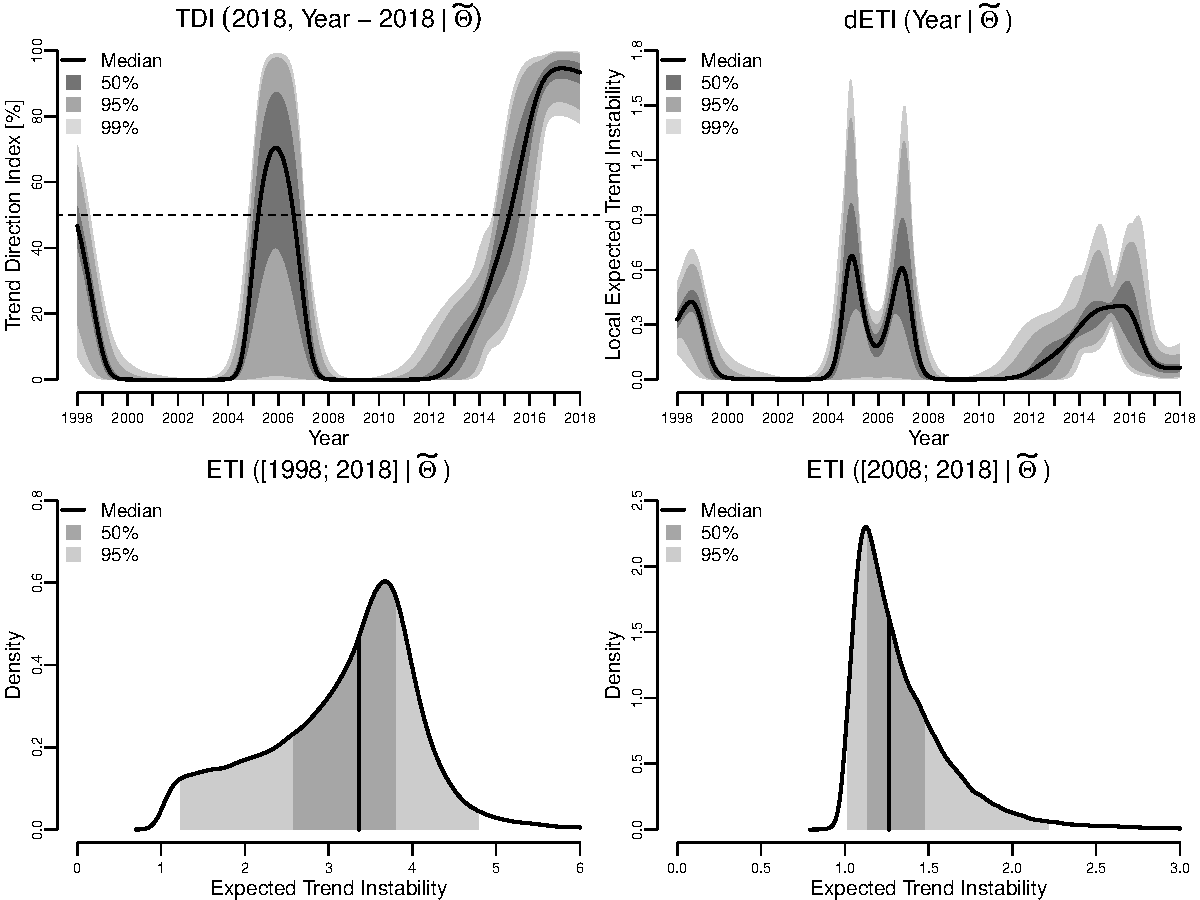
\includegraphics{bayesFitPlot}
\caption{Results from fitting the latent Gaussian process model by Bayesian analysis. The first row shows the posterior distributions of TDI (left) and local ETI (right) with the posterior means in bold and gray areas showing point-wise 95$\%$ and 99$\%$ probability intervals for the posterior distribution. The second row shows densities and probability intervals for the expected trend instability for the 20-year period back-in-time from 2018 (left) and 10 year back-in-time (right).}
\label{fig:bayesFitPlot}
\end{figure}

\begin{table}[htbp]
\center
\begin{tabular}{l|rrr}
  & Maximum Likelihood & \multicolumn{2}{l}{Bayesian Posterior}\\ \hline
$\text{TDI}(2018, 0)$  & 95.24\% & 93.32\% & $[82.15\%; 98.86\%]$\\
$\text{TDI}(2018, -1)$ & 95.92\% & 94.21\% & $[84.28\%; 99.11\%]$\\
$\text{TDI}(2018, -2)$ & 74.41\% & 77.87\% & $[51.02\%; 94.94\%]$\\
$\text{TDI}(2018, -3)$ & 33.36\% & 44.11\% & $[18.23\%; 69.19\%]$\\
$\text{TDI}(2018, -4)$ & 18.96\% & 20.60\% & $[6.05\%; 31.82\%]$\\
$\text{TDI}(2018, -5)$ & 9.50\% & 6.21\% & $[0.03\%; 22.21\%]$\\ \hline
Crosspoint & 2015.48 & 2015.19 & $[2014.62; 2015.96]$\\ \hline
$\text{ETI}([1998, 2018])$ & 3.68 & 3.36 & $[1.24; 4.79]$\\
$\text{ETI}([2008, 2018])$ & 1.39 & 1.25 & $[1.02; 2.22]$
\end{tabular}
\caption{Summary measures from the Maximum Likelihood and Bayesian analyses. The rows show the estimated Trend Direction Index for 2013 to 2018 and the Expected Trend Instability for the last 10 and 20 years all conditional on data from 1998 to 2018. For the Bayesian analysis posterior medians and 95$\%$ posterior probability intervals are given. Crosspoint is the time during the last $10$ years where $\mathrm{TDI}$ first exceeded $50\%$.}
\label{tab:summaries}
\end{table}

The results from the two analyses generally agree, but there are two
differences that we wish to address. Both analyses showed a local peak
in trendiness around 2015. In the maximum likelihood analysis this
occurred at 2005.94 with a Trend Direction Index of \(86.47\%\). In the
Bayesian analysis the peak occurs at 2005.87 with a median Trend
Direction Index of \(79.43\%\) and a \(95\%\) posterior probability
interval of \([1.23\%; 97.73\%]\). The added uncertainty estimates
facilitated by the Bayesian estimator shows this trendiness is so
variable that there is no reason to believe in a substantial increase in
proportions at that point in time. This insight could not have been
obtained from the maximum likelihood analysis.

The second difference is that the Bayesian model seems to generally
induce more sluggish estimates due to mixing over the underlying
parameters. This can be seen from the plot of the median local Expected
Trend Instability in Figure \ref{fig:bayesFitPlot} which is generally
lower than its corresponding maximum likelihood point estimates in
Figure \ref{fig:likFitPlot}. This is similarly reflected in the median
ETI estimates in Table \ref{tab:summaries} which are lower than their
values under maximum likelihood. Looking at the posterior distributions
of the covariance parameters \(\theta\) (not shown), we see that this is
mainly a result of not restricting the parameter \(\nu\) to its maximum
likelihood value. The 95\% probability interval of the posterior
distribution of \(\nu\) was \([0.328; 10.743]\) which is highly
right-skewed compared to the maximum likelihood estimate of
\(\widehat{\nu^\text{ML}} = 1.020\).

To understand the effect of \(\nu\) on the smoothness of the fitted
models we can compare the local expected number of crossings by a
Gaussian process and its derivative at their mean values in the simple
case of a zero-mean process with either the Rational Quadratic or the
Squared Exponential covariance function. In this case the formula in
Proposition \ref{prop:ETIposterior} simplifies immensely, and as shown
in the supplementary material the local expected number of
mean-crossings by \(f\) is equal to \(\pi\rho^{-1}\) for both covariance
functions. However, for \(df\) the local expected number of
mean-crossings is equal to \(3^{1/2}\pi^{-1}\rho^{-1}\) for the Squared
Exponential covariance function and
\(3^{1/2}\pi^{-1}\rho^{-1}(1 + \nu^{-1})^{1/2}\) for the Rational
Quadratic covariance function. We note that
\(1 < (1 + v^{-1})^{1/2} < \infty\) for \(0 < \nu < \infty\) and
monotonically decreasing for \(\nu \rightarrow \infty\) with a limit of
one. Therefore, the value of \(\nu\) has no effect on the crossing
intensity of the process itself, but its derivative is always larger
under a Rational Quadratic covariance function compared to the Squared
Exponential covariance function with equality in the limit. A
right-skewed posterior distribution of \(\nu\) therefore favors fewer
crossings of the trend leading to a more stable trend and a smaller
value of the Expected Trend Instability.

\section{Discussion}\label{sec:discussion}

In this article, we have proposed two new measures - the Trend Direction
Index and the Expected Trend Instability - in order to quantify the
behavior of an underlying trend. Using a Gaussian process model for the
latent structure we show how the TDI and the ETI can be estimated from
data in both a maximum likelihood and a Bayesian framework and provide
probabilistic statements about the monotonicity of the latent trend.

Both indices have an intuitive interpretation that directly refers to
properties of the latent trend and the proposed approach exploits the
underlying assumed continuity to circumvent discretization and allows us
to compute a different (and more relevant) probability than what can be
obtained from e.g., a \(\chi^2\) test.

It is worth noting that the indices are scale-free and thus they do not
tell anything about the magnitude of a trend. Consequently, the two
indices should therefore always be accompanied by plots of the posterior
of \(df\). If a prespecified size of a trend change, \(u\), is desired
then the threshold in the definition of the TDI is easily modified to
accommodate this in the definition of the TDI:

\begin{align*}
  \mathrm{TDI}_u(t, \delta) = P(df(t + \delta) > u \mid \mathcal{F}_t), \quad t \in \mathcal{T}.
\end{align*}

In conclusion, we have introduced a method for evaluation of trends that
specifically address questions such as ``Has the trend changed?''. Our
approach is based on two intuitive measures that are easily interpreted,
provide well-defined measures of trend behavior and which can be applied
to a large number of situations. The flexibility of the model is further
improved by the minimum of assumptions necessary to provide about the
underlying latent trend.

\section{Bibliography}\label{bibliography}

\hypertarget{refs}{}
\hypertarget{ref-barry1993bayesianchangepoint}{}
Barry, Daniel, and J. A. Hartigan. 1993. ``A Bayesian Analysis for
Change Point Problems.'' \emph{Journal of the American Statistical
Association} 88 (421). {[}American Statistical Association, Taylor \&
Francis, Ltd.{]}: 309--19. \url{http://www.jstor.org/stable/2290726}.

\hypertarget{ref-bassemand1993abrupt}{}
Basseville, Michele, and Igor V. Nikiforov. 1993. \emph{Detection of
Abrupt Changes: Theory and Application}. Prentice-Hall.

\hypertarget{ref-carlstein1994change}{}
Carlstein, Edward, Hans-Georg Müller, and David Siegmund, eds. 1994.
\emph{Change-Point Problems}. Vol. 23. Lecture Notes -- Monograph
Series. Institute of Mathematical Statistics.

\hypertarget{ref-carpenter2017stan}{}
Carpenter, Bob, Andrew Gelman, Matthew D Hoffman, Daniel Lee, Ben
Goodrich, Michael Betancourt, Marcus Brubaker, Jiqiang Guo, Peter Li,
and Allen Riddell. 2017. ``Stan: A Probabilistic Programming Language.''
\emph{Journal of Statistical Software} 76 (1).

\hypertarget{ref-chandler2011statistical}{}
Chandler, R., and M. Scott. 2011. \emph{Statistical Methods for Trend
Detection and Analysis in the Environmental Sciences}. Statistics in
Practice. Wiley.

\hypertarget{ref-cramer1967stationary}{}
Cramer, Harald, and M. R. Leadbetter. 1967. \emph{Stationary and Related
Stochastic Processes -- Sample Function Properties and Their
Applications.} John Wiley \& Sons, Inc.

\hypertarget{ref-esterby1993trenddef}{}
Esterby, S. R. 1993. ``Trend Analysis Methods for Environmental Data.''
\emph{Environmetrics} 4 (4): 459--81.
doi:\href{https://doi.org/10.1002/env.3170040407}{10.1002/env.3170040407}.

\hypertarget{ref-gelman1992inference}{}
Gelman, Andrew, and Donald B. Rubin. 1992. ``Inference from Iterative
Simulation Using Multiple Sequences.'' \emph{Statistical Science} 7 (4):
457--72.

\hypertarget{ref-gottlieb2012stickiness}{}
Gottlieb, Andrea, and Hans-Georg Müller. 2012. ``A Stickiness
Coefficient for Longitudinal Data.'' \emph{Computational Statistics \&
Data Analysis} 56 (12): 4000--4010.

\hypertarget{ref-gptrendStan}{}
Jensen, Andreas Kryger. 2019. ``GitHub Repository for the Trendiness of
Trends.'' \url{https://github.com/aejensen/TrendinessOfTrends}.

\hypertarget{ref-politiken}{}
Navne, Helene, Anders Legarth Schmidt, and Lars Igum Rasmussen. 2019.
``Første Gang I 20 år: Flere Danskere Ryger.''
\url{https://politiken.dk/forbrugogliv/sundhedogmotion/art6938627/Flere-danskere-ryger}.

\hypertarget{ref-quandt1958estimation}{}
Quandt, Richard E. 1958. ``The Estimation of the Parameters of a Linear
Regression System Obeying Two Separate Regimes.'' \emph{Journal of the
American Statistical Association} 53 (284): 873--80.

\hypertarget{ref-R-Core-Team:2018aa}{}
R Core Team. 2018. \emph{R: A Language and Environment for Statistical
Computing}. Vienna, Austria: R Foundation for Statistical Computing.
\url{https://www.R-project.org/}.

\hypertarget{ref-neal1999regression}{}
Radford, Neal M. 1999. ``Regression and Classification Using Gaussian
Process Priors (with Discussion).'' In \emph{Bayesian Statistics 6:
Proceedings of the Sixth Valencia International Meeting}, edited by A.
P. Dawid José M. Bernardo James O. Berger and Adrian F. M. Smith,
475--501.

\hypertarget{ref-rasmussen2003gaussian}{}
Rasmussen, C. E., and C. K. I. Williams. 2006. \emph{Gaussian Processes
in Machine Learning}. MIT Press.

\hypertarget{ref-rstan}{}
Stan Development Team. 2018. ``RStan: The R Interface to Stan.''
\url{http://mc-stan.org/}.

\hypertarget{ref-sst}{}
The Danish Health Authority. 2019. ``Danskernes Rygevaner 2018.''
\url{www.sst.dk/da/udgivelser/2019/danskernes-rygevaner-2018}.


\end{document}
